%************************************************
\chapter{Introduction}\label{ch:introduction}
%************************************************
\section{Introduction}
Navigation and planning are essential for mobile robots to act in out- and indoor environments. 
From self driving cars navigating 132~miles through the Mojave desert, or mobile robots handling goods in distribution centers and warehouses to mobile robots used for planetary exploration, autonomous robots have conquered nearly every place on earth and beyond.
 
Articles like \cite{stanley} and \cite{kiva} present the relationship between the environmental complexity and the computational on-board processing power needed to tackle the navigation problem.
The self driving car Stanley has a six processor computing platform provided by Intel whilst Kiva robots are using low cost DSP's for navigation and vision processing\footnote{Kiva Systems Uses "Smart" Blackfin-powered Robots for Warehouse Navigation | Analog Devices: \url{http://www.analog.com/en/content/kiva_systems_bf548/fca.html}} to drive within a known environment.  

While the application domains and computational powers varies strongly between the robotic systems, all of them have to move safely and efficient from one location to another.   
In order to give an impression of the importance of navigation and planning in the field of mobile robotics the next section gives some motivation and application examples.

\section{Motivation and Applications}\label{sec:motivation} 
The goal of navigation encompasses the ability of robots to find a series of actions based on its knowledge of the environment and sensor values to reach its goal position in an effective and efficient manner.
The resulting series of actions is called a \emph{plan}. 

To ensure safety and flexibility in the presence of obstacles in a dynamic environment \emph{obstacle avoidance} is used to alter plans during execution and generating of collision free trajectories.

A common strategy to deal with complex navigation problems is to the divide the planning task into a global and a local planning problem \cite{LaValle2006}.

Global path-planning usually operates on a simplified representation of the environment and the robot itself (e.g. static map, circle representation of the robots outline) to efficiently compute an optimal shortest path using variants of Dijkstra's \cite{dijkstra1959note} or $A^*$ \cite{DBLP:journals/tssc/HartNR68/Astar} algorithm, ignoring kinematic and acceleration constraints of the robot.
In succession the retrieved global path is used by a local planner for guiding the robot through the environment.
Figure~\ref{fig:fig_pioneer} illustrates the view of the environment from a robot perspective together with a global and local plan, which enables the robot to drive autonomous within our lab/office environment.

\begin{figure}[thpb]
      \centering
      \def\svgwidth{\textwidth}
      \includesvg{figures/pioneer_costmap}
      \caption[Global and local planning.]{This figure shows a Pionner3DX and its view of the office environment while passing through a door. The blue line shows the global path and the green line the selected trajectory of the local planner.}
      \label{fig:fig_pioneer}
\end{figure}

The major responsibility for local planner is obstacle avoidance. It takes sensor readings of the robot into account and is reactive to changes within the sensor range. 
It selects the best values of available motor controls in respect to the kinematic and dynamic constraints of the robot, generating collision free trajectories. 
   
Navigation competence is essential for a broad spectrum of application domains within the field of mobile robotics which are presented below:

\begin{description}
\item[Self driving cars]\hfill \\
Self driving cars (see Figure~\ref{fig:fig_auto}) like Stanley \cite{stanley} which won the 2005 DARPA Grand Challenge and the Google car \cite{guizzo2011google} are two examples which illustrate the enormous potential of autonomous vehicles.
While the former is confronted with rough terrain and manoeuvrs at high speeds, cars in urban traffic have to be prepared for other vehicles, pedestrians and have to incorporate traffic rules into the navigation task. 

\begin{figure}[thpb]
	  \myfloatalign
      \footnotesize
      \centering
    \subfloat[Stanley (taken from \cite{stanley}).]
    {  \label{fig:fig_stanley}
        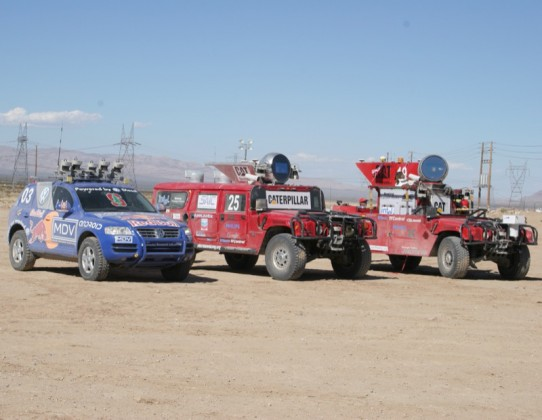
\includegraphics[width=0.45\textwidth,height=0.2\textheight]{figures/fig_stanley.jpg}
    }    
    \subfloat[Google car (Credit: Google\protect\footnotemark).]
    {  \label{fig:fig_googlecar}
       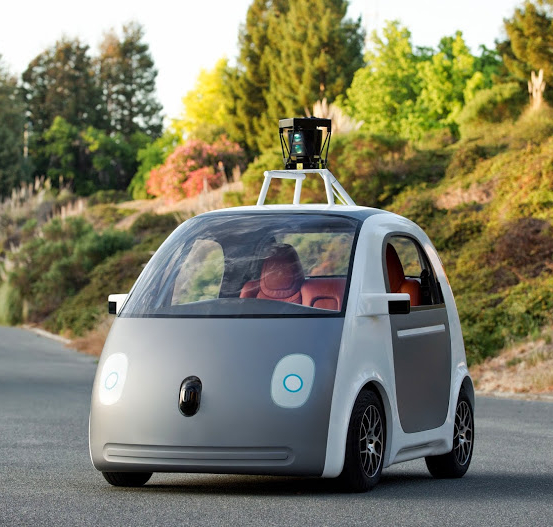
\includegraphics[width=0.45\textwidth,height=0.2\textheight]{figures/fig_googlecar.jpg}
    }
   \caption[Selfdriving car]{Self driving cars designed for different environments. On the left the winner of the 2005 DARPA Grand Challenge tackled wreckless driving through the Mojave desert and the right picture shows the new Google car designed for urban traffic.}
   \label{fig:fig_auto}
\end{figure}

\item[Planetary exploration]\hfill \\
Another example of autonomous vehicles are planetary rovers.
Three generations of Mars rovers developed at NASA are shown in Figure~\ref{fig:fig_nasa}. 
The first Mars rover, Sojourner, which landed on Mars in 1997 as part of the Mars Pathfinder Project was remotely operated from earth. 
The next generation of rovers, Spirit and Opportunity which landed 2004, did already have an autonomous navigation system. This enabled the robots to avoid hazardous situations without human intervention. 
The latest rover Curiosity is on its mission on Mars since August 2012 using autonomous navigation to explore mars on safe paths without the help of human rover drivers.

An overview of recent developments in the field of planetary exploration including navigation topics can be found in \cite{PavoneAcikmese2014rover}.

\begin{figure}[thpb]
	  \myfloatalign
      \footnotesize
      \centering
    \subfloat[NASA Mars rover (Credit: NASA JPL-Caltech).]
    {  \label{fig:fig_nasa}
        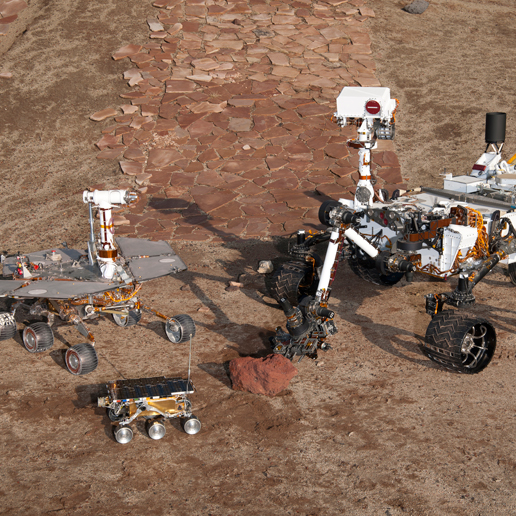
\includegraphics[width=0.45\textwidth,height=0.2\textheight]{figures/fig_marsrover.jpg}
        %\caption{Dijkstra}
    }
    \subfloat[Mawson rover (taken from \cite{Allister2012rover}).]
    {  \label{fig:fig_rover}
        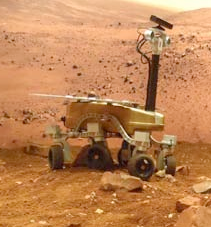
\includegraphics[width=0.45\textwidth,height=0.2\textheight]{figures/fig_rover.png}
        %\caption{Dijkstra}
    }     
   \caption[Mars rover]{Different Mars rover for planetary exploration. On the left Sojourner, Spirit and Curiosity from NASA which provided rich scientific information exploring Mars and on the right Mawson an academic research project on a training track at the Museum of Sydney.}
   \label{fig:fig_rover}
\end{figure}
\footnotetext{Google self driving car available from \url{http://googleblog.blogspot.co.at/2014/05/just-press-go-designing-self-driving.html}}

\item[Search and Rescue]\hfill \\
Mobile robots provide a useful tool for rescue teams, whenever human intervention is not possible due to imminent risk of health and life, like immediate explosion hazard or threat of nuclear radiation.  
Figure~\ref{fig:fig_rescue} shows two prominent representatives of search and rescue robots.
\begin{figure}[thpb]
	  \myfloatalign
      \footnotesize
      \centering
    \subfloat[Pioneer (Credit: Carnegie Mellon University)]
    {  \label{fig:fig_chernobyl}
        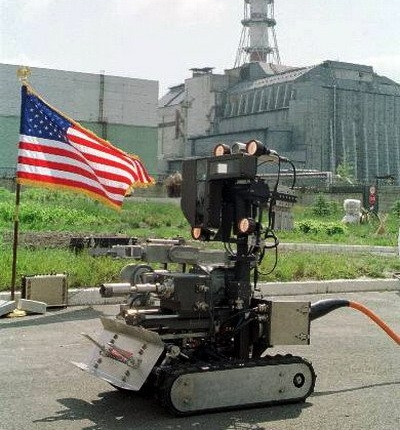
\includegraphics[width=0.45\textwidth,height=0.2\textheight]{figures/fig_chernobyl_pioneer.jpg}
        %\caption{Dijkstra}
    }
    \subfloat[Packbot (Credit: iRobot)]
    {  \label{fig:fig_fukushima}
        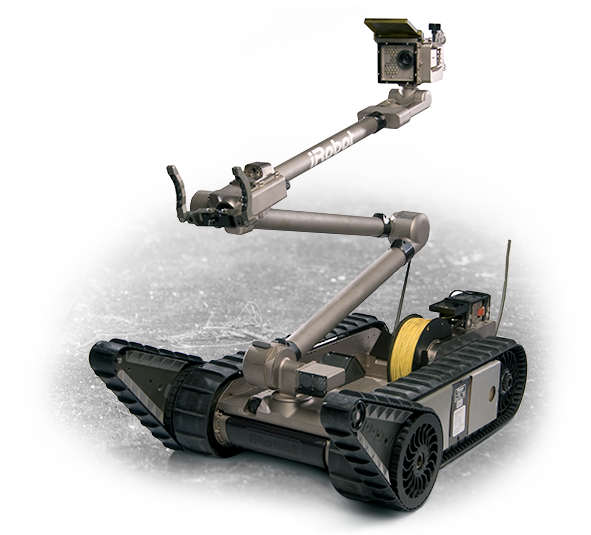
\includegraphics[width=0.45\textwidth,height=0.2\textheight]{figures/fig_packbot.png}
        %\caption{Dijkstra}
    }     
   \caption[Rescue robots]{PIONNEER in chernobyl and PACKBOT in Fukushima.}
   \label{fig:fig_rescue}
\end{figure}

The robot PIONEER sponsored by the US Department of Energy and NASA was the first of its kind to be deployed to the remnants of the nuclear power station in Chernobyl in the Ukraine after the supergau in 1986. 
The robots mission was to evaluate the sarcophagus which was built to shield off radiation.

In 2011 after an earthquake caused a nuclear disaster at the Fukushima Daiichi power plant in Japan, two PACKBOT robots of the American company iRobot were deployed to perform on site observations.

While the aforementioned robots were remotely operated, autonomous robots are a hot research topic in this domain and already provide impressive results like Hector the winner of the 2014 RoboCup Rescue League \cite{2014:hector_rescue_tdp}.

\item[Logistics and Transportation]\hfill \\
Automated guided vehicles (AGV) are an essential part in industry to support automated manufacturing. Figure~\ref{fig:fig_agv} shows a typical AGV from the Austrian company DS-Automotion.
The mobile robots follow markers, wires, or magnets in the floor, and make use of lasers and computer vision methods to accomplish navigation tasks. 
Their main responsibility is to move materials safely and efficient around manufacturing facilities, warehouses (eg. Kiva Systems \cite{kiva}) or hospitals (eg. HELPMATE \cite{ROB:4520696}). 

If transportation by road is not possible a flying drone might do the job. Projects from major companies like Googles \emph{project wing}\footnotetext{Google self driving delivery drones \url{https://plus.google.com/+google/posts/TqrsvRyPeNH}} and Amazons \emph{Prime Air} are working on self flying drones to deliver packages. 
Figure~\ref{fig:fig_uav} shows a prototype drone on a test flight. 

\begin{figure}[thpb]
	  \myfloatalign
      \footnotesize
      \centering
    \subfloat[AGV (Credit: DS-Automotion)]
    {  \label{fig:fig_agv}
        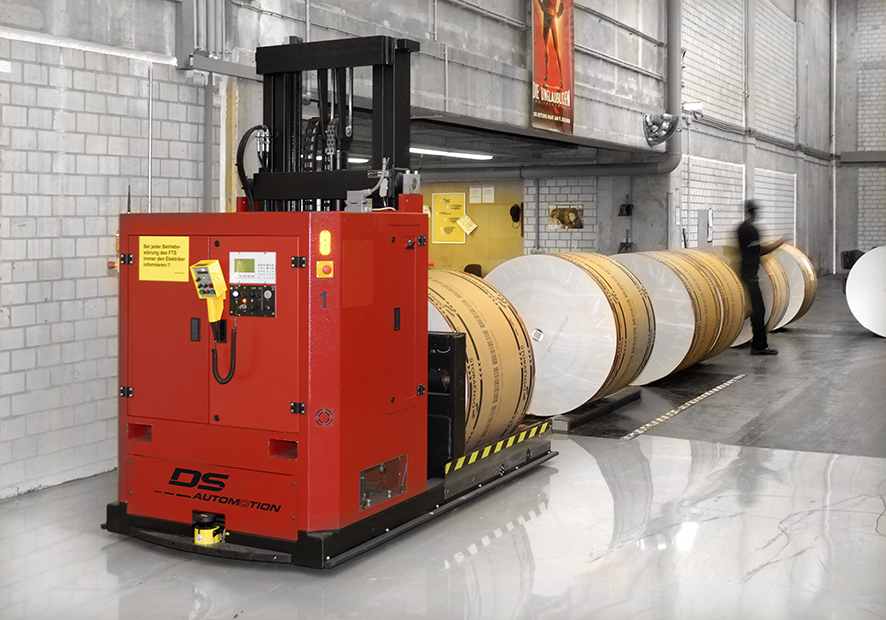
\includegraphics[width=0.45\textwidth,height=0.2\textheight]{figures/fig_AGV-dsautomation.jpg}
        %\caption{Dijkstra}
    }
    \subfloat[Project Wing delivery drone (Credit: KEYSTONE)]
    {  \label{fig:fig_uav}
        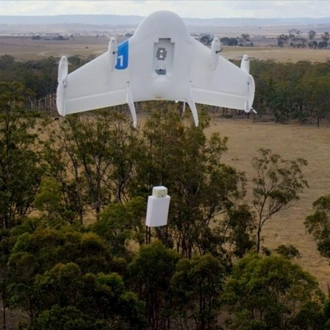
\includegraphics[width=0.45\textwidth,height=0.2\textheight]{figures/fig_wing.jpg}
        %\caption{Dijkstra}
    }     
   \caption[Logistic robots]{Transportation on earth using Automated Guided Vehicles and in the air with the support of self flying drones.}
   \label{fig:fig_transport}
\end{figure}

\item[Assistance and Companion Robots]\hfill \\
Companion KIBA, 
Health Care HOBBIT \cite{fischinger2013hobbit}, 
Guide RHINO, ROBOX \cite{philippsen:2004:phd}
\begin{figure}[thpb]
	  \myfloatalign
      \footnotesize
      \centering
    \subfloat
    {  \label{fig:fig_agv}
        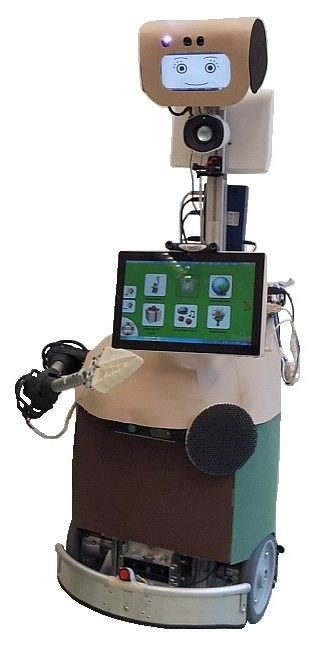
\includegraphics[width=0.45\textwidth,height=0.4\textheight]{figures/fig_hobbit.png}
        %\caption{Dijkstra}
    }
    \subfloat
    {  \label{fig:fig_uav}
        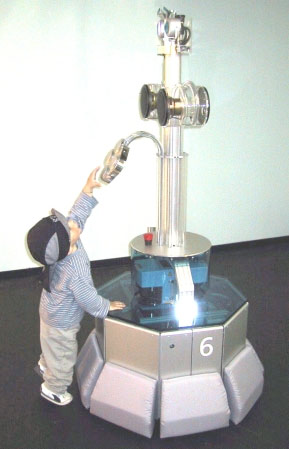
\includegraphics[width=0.45\textwidth,height=0.4\textheight]{figures/fig_robox.png}
        %\caption{Dijkstra}
    }     
   \caption[Assitance robots]{Hobbit a care robot to support elderly people and Robox a museum tour guide.}
   \label{fig:fig_rescue}
\end{figure}


\item[Commercial]\hfill \\
Mining Robots, law mowing, floor cleaning, harvesting
FRANC and ARW Paper
inpipe robot \cite{mateos2013inpipe}
crop robot \cite{Schuetz2014}
\begin{figure}[thpb]
	  \myfloatalign
      \footnotesize
      \centering
    \subfloat
    {  \label{fig:fig_agv}
        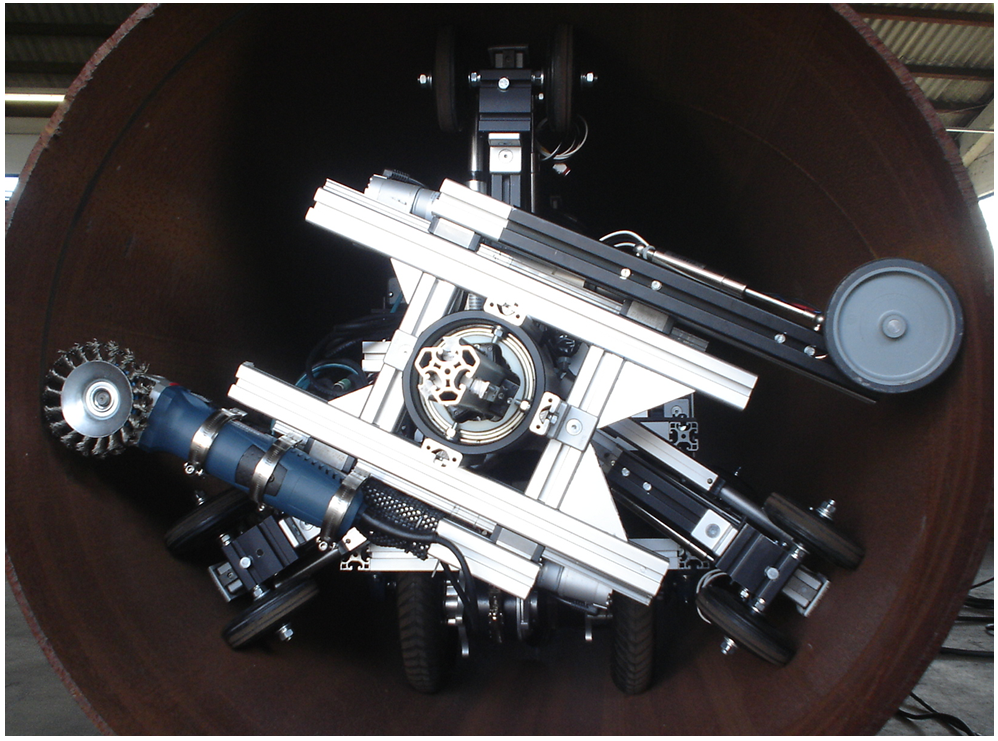
\includegraphics[width=0.45\textwidth,height=0.2\textheight]{figures/fig_inpiperobot.png}
        %\caption{Dijkstra}
    }
    \subfloat
    {  \label{fig:fig_uav}
        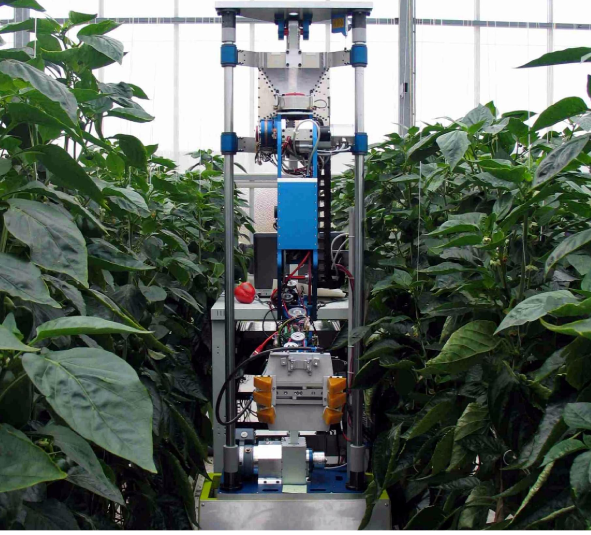
\includegraphics[width=0.45\textwidth,height=0.2\textheight]{figures/fig_croprobot.png}
        %\caption{Dijkstra}
    }     
   \caption[Commercial robots]{The right figure shows an in-pipe maintenance robot, the left image an agricultural robot used for harvesting crops.}
   \label{fig:fig_rescue}
\end{figure}

\item[Challenges and Competitions]\hfill \\
FIRA
Robocup,Robotsoccer Standard platform League, other Leagues
FIRA3 and RoboCup 4 are two organizations intended to promote robot soccer. They
attempt to provide a standard problem where wide ranges of technologies must be combined
and integrated.
Federation of International Robot-soccer Association, founded in 1997. Details can be found at www.fira.net
RoboCup Federation, founded in 1993. Details can be found at www.robocup.org.

Robot@Home
RobocupLogisticLeague
DARPA

\end{description}

Other fields not in robotic environment. Knot entangling puzzles, automation and assembly, Molecular biology and medicine.
And a short summary towards the goal of the thesis.

\section{Goal of Thesis and Scientific Contribution}\label{sec:goal}


One of the most popular local planer and reactive collision avoidance method is the Dynamic Window Approach (DWA)\cite{DWA1997}. Its based on evaluating a fixed number of trajectory samples in a reduced velocity space. 
A dynamic window around the current robot fused with the current sensor readings of the robot represents a so called costmap.
Trajectories are sampled into that costmap and weighted by a cost function.
Recent adoptions of this method can be found in \cite{conf/icra/SederP07}\cite{DBLP:conf/icra/Marder-EppsteinBFGK10}

In this paper we propose a method which finds the best velocity commands by using search strategies based on Meta-Heuristics instead of evaluating a fixed number of trajectories in a brute force manner.
A combination of Iterated Local Search (ILS) with different neighborhood structures, Variable Neighborhood Search (VNS), and a Tabu list provides a significant documented performance boost. 

This enables the local planer to:
\begin{itemize}
\item run at a higher frequency
\item simulate trajectories for a longer time interval
\item moving the robot at higher speed
\item investigate a larger amount of trajectories
\item use a higher costmap resolution
\end{itemize}

\section{Outline}\label{sec:outline}
This work is structured in the following way. 
In Chapter \ref{ch:introductionplanning} the basic sources for planning are outlined, covering the basic problem definition, representation of the environment and different robotic motion models. 

Chapter \ref{ch:planningalgorithms} gives an overview of important planning algorithms and obstacle avoidance methods.
 
Chapter \ref{ch:meta} represents the main part of this thesis and introduces meta-heuristic extensions to local planning methods. 
Starting with an detailed overview of  meta-heuristic algorithm, two application based on ILS and VNS are used for trajectory selection of a local planner and described in Section \ref{sec:trajselmeta}.

A detailed evaluation of these methods is presented in Chapter \ref{ch:eval}, using a very simple implementation of a local planner and randomly generated sensor maps. 
The gathered data is then used to implement a meta-heuristic trajectory selection in a high sophisticated planner and tested using simulation software with a robust physical engine.

Chapter \ref{ch:conc} concludes the work of this thesis with a short summary and an outlook on future research directions.
%*****************************************
%*****************************************
%*****************************************
%*****************************************
%*****************************************




